\section{Introduction}

This chapter presents OmniTune, a set of interfaces for designing
extensible, distributed autotuners, capable of runtime prediction of
optimisation parameters using machine learning. OmniTune supports
collaborative, online learning of optimisation spaces. I first
describe the basic approaches to predicting optimisation parameters
that OmniTune supports, followed by a description of the architecture
and public interfaces exposed by OmniTune.


\section{System Architecture and Interface}

\begin{figure}
\centering
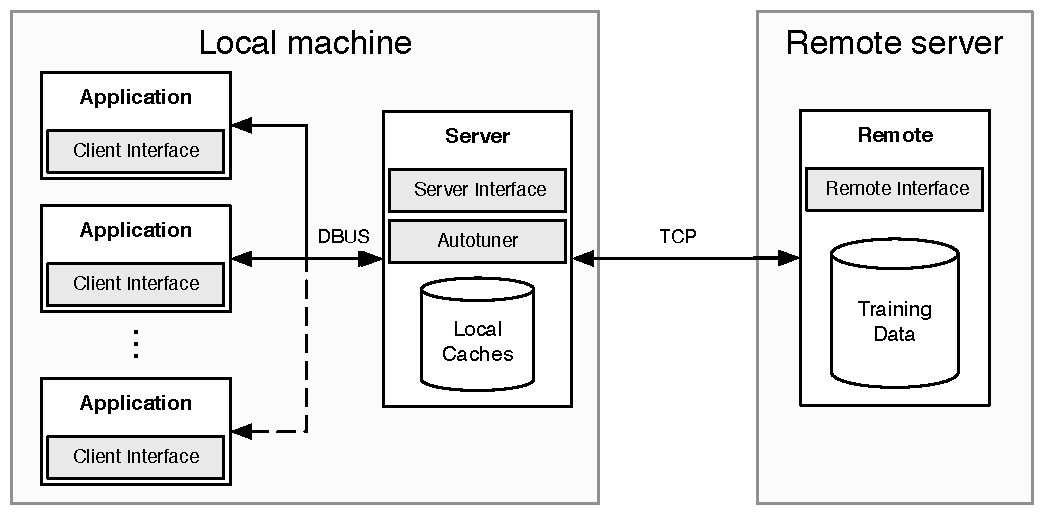
\includegraphics[width=.9\textwidth]{img/omnitune-system-overview.pdf}
\caption{%
  High level overview of OmniTune.%
}
\label{fig:omnitune-system-overview}
\end{figure}

Omnitune is built around a three tier client-server model, illustrated
in Figure~\ref{fig:omnitune-system-overview}. The goal is to separate
the concerns of application-specific and autotuning logic. In
OmniTune, the applications which are to be autotuned are referred to
as \emph{clients}. These clients commmunicate with a system-wide
\emph{server}, which handles autotuning requests from clients. The
server caches data sourced from a \emph{remote}, which maintains a
global store of all training data.

As discussed in \xref{related work}, common implementations of
autotuning in the literature either: embed the autotuning logic within
the each target application, or take a standalone approach in which
the autotuner is a program which must be invoked by the user to tune a
target application. Embedding the autotuner within each target
application has the advantage of providing ``always-on'' behaviour,
but is infeasible for complex systems in which the cost of building
machine learning model must be added to each program run. The
stanadlone approach separates the autotuning logic, at the expense of
adding one additional step to the build process. The approach taken in
OmniTune aims to capture the advantages of both techniques by
implementing an autotuning service with communication logic embedded
in the target applications. The resulting design consists of three
sets of components: clients, servers, and a remote data-store.

There is a many to one relationship between clients, servers, and
remotes, such that a single remote may handle connections to multiple
servers, which in turn may accept connections from multiple
clients. This design has two primary advantages: the first is that it
decouples the autotuning logic from that of the client program,
allowing developers to easily repurpose the autotuning framework to
target additional optimisation parameters without a significant
development overhead for the target applications; the second advantage
is that this enables collective tuning, in which training data
gathered from a range of devices can be accessed and added to by any
OmniTune server.

OmniTune supports autotuning using a separate offline training phase,
online training, or a mixture of both. Figure~\ref{fig:omnitune-comms}
shows an example pattern of communication between the three tiers of
an OmniTune system, showing a distinct training phase. Note that this
training phase is enforced only by the client. The following sections
describe the interfaces between the three components.


\begin{figure}
\centering
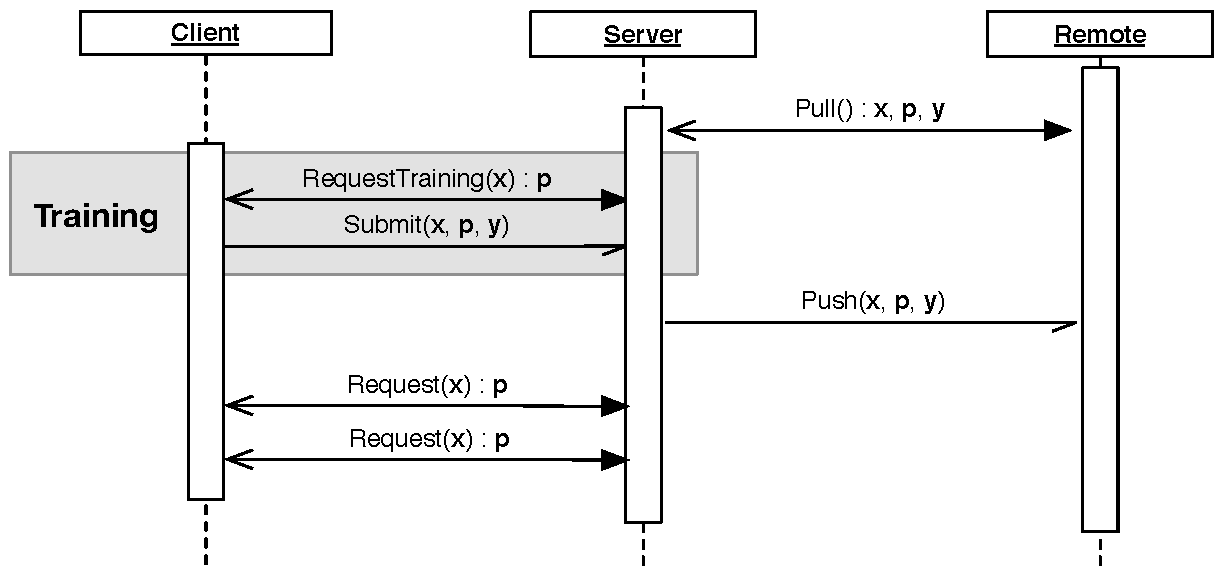
\includegraphics[width=\textwidth]{img/omnitune-comms.pdf}
\caption{%
  An example communication pattern between OmniTune components,
  showing an offline training phase.%
}
\label{fig:omnitune-comms}
\end{figure}


\subsection{Client Interface: Lightweight Communication}

Client applications communicate with an OmniTune server through four
operations:

\begin{itemize}
\item \textsc{Request}$(x) \to p$ Given a set of explanatory variables
  $x$, request a set of parameter values $p$ to maximise performance.
\item \textsc{RequestTraining}$(x) \to p$ Given a set of explanatory
  variables $x$, allow the server to select a set of parameter values
  $p$ for evaluating their fitness.
\item \textsc{Submit}$(x, p, y)$ Submit an observed measurement of
  fitness $y$ of parameters $p$, given explantory variables $x$.
\item \textsc{Refuse}$(x, p)$ Refuse a set of parameters $p$ given a
  set of explanatory variables $x$. Once refused, those parameters
  will not be returned by any subsequent calls to \textsc{Request()}
  or \textsc{RequestTraining()}.
\end{itemize}

This set of operations enables the core functionality of an autotuner,
while providing flexibility for the client to control how and when
training data is collected.


\subsection{Server: Autotuning Engine}

For each autotuning-capable machine, a system-level daemon hosts a
DBus session bus which client processes communicate with. This daemon
acts as an intermediate between the training data and the client
applications, \emph{serving} requests for optimisation parameter
values. Servers operations are application-specific, so there is a set
of operations to implement autotuning of each supported optimisation
target.

The server is implemented as a standalone Python program, and contains
a library of machine learning tools to perform parameter prediction,
interfacing with Weka\footnote{http://www.cs.waikato.ac.nz/ml/weka/}
using the JNI. Servers may perform additional feature extraction of
explanatory variables supplied by incoming client requests. The reason
for performing feature extraction on the server as opposed to on the
client side is that this allows the results of expensive operations
(for example, analysing source code of target applications) to be
cached for use across the lifespan of client applications. These
caches are synced with the remote to

On launch, the server requests the latest training data from the
remote, which it uses to build the relevant models for performing
prediction of optimisation parameter values. Servers communicate with
remotes by submitting or requesting training data in batches, using
two operations:

\begin{itemize}
\item \textsc{Push}$(\bf{f}, \bf{c})$ Submit a set of labelled training
  points as pairs $(f,c)$.
\item \textsc{Pull}$() \to (\bf{f}, \bf{c})$ Request training data as a
  set of labelled $(f,c)$ pairs.
\end{itemize}


\subsection{Remote: Distributed Training Data}

\TODO{\ldots}


\section{Predicting Optimisation Parameter Values}

Figure~\ref{fig:omnitune-system-flow} shows the \TODO{\ldots}

% Predicting values for optimisation parameters

% separate training phase


\begin{figure}
\centering
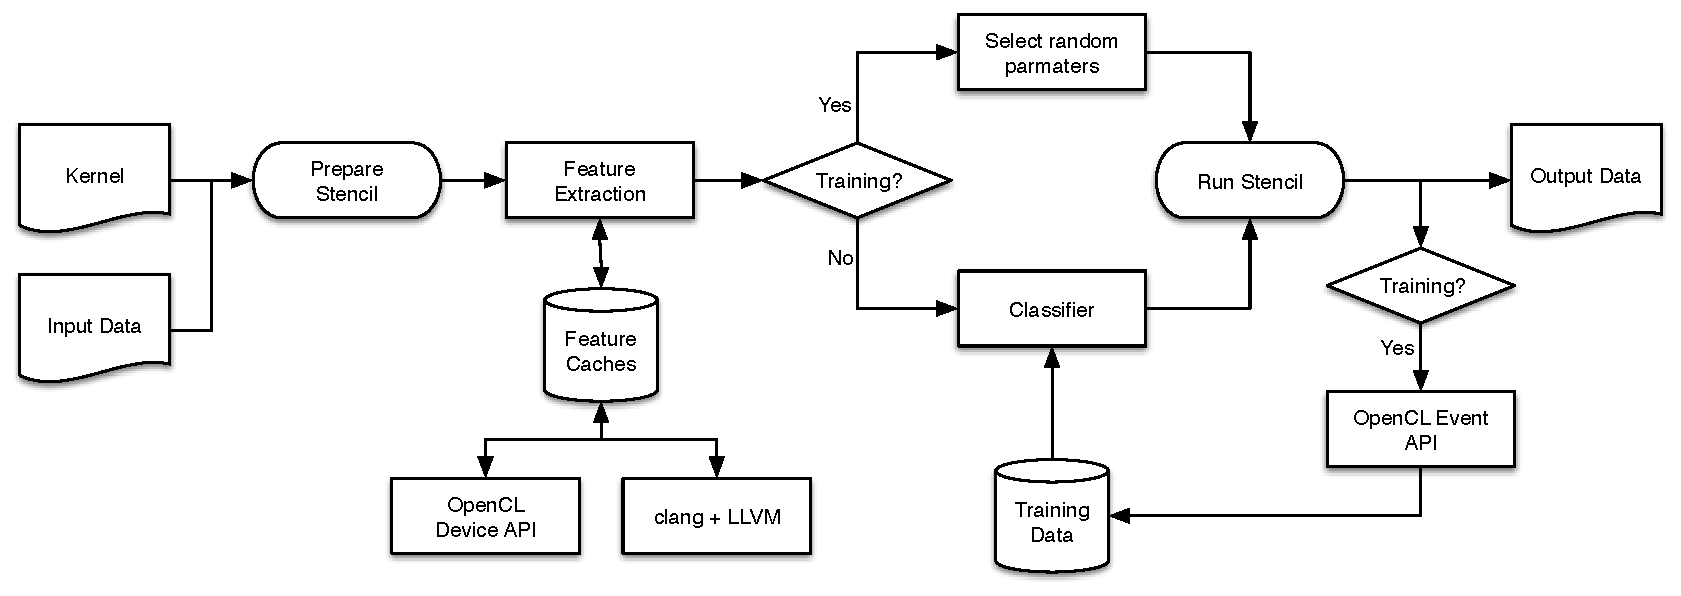
\includegraphics[width=\textwidth]{img/omnitune-system-flow.pdf}
\caption{%
  Selecting optimisation parameter values with OmniTune.%
}
\label{fig:omnitune-system-flow}
\end{figure}


\section{Summary}

This chapter has described the architecture of of OmniTune, a
distributed autotuner which is capable of performing runtime
prediction of optimal workgroup sizes using a variety of machine
learning approaches. OmniTune uses a client-server model to decouple
the autotuning logic from target programs and to maintain separation
of concerns. It uses lightweight inter-process communication to
achieve low latency autotuning, and uses caches and lookup tables to
minimise the one-off costs of feature extraction.
